\documentclass[tikz,convert={convertexe={magick},outext=.png}]{standalone}
\usepackage{tikz}
\usepackage{pgfplots}
\usepackage{amsmath}
\pgfplotsset{compat=1.18}
\usepgfplotslibrary{fillbetween}

\begin{document}
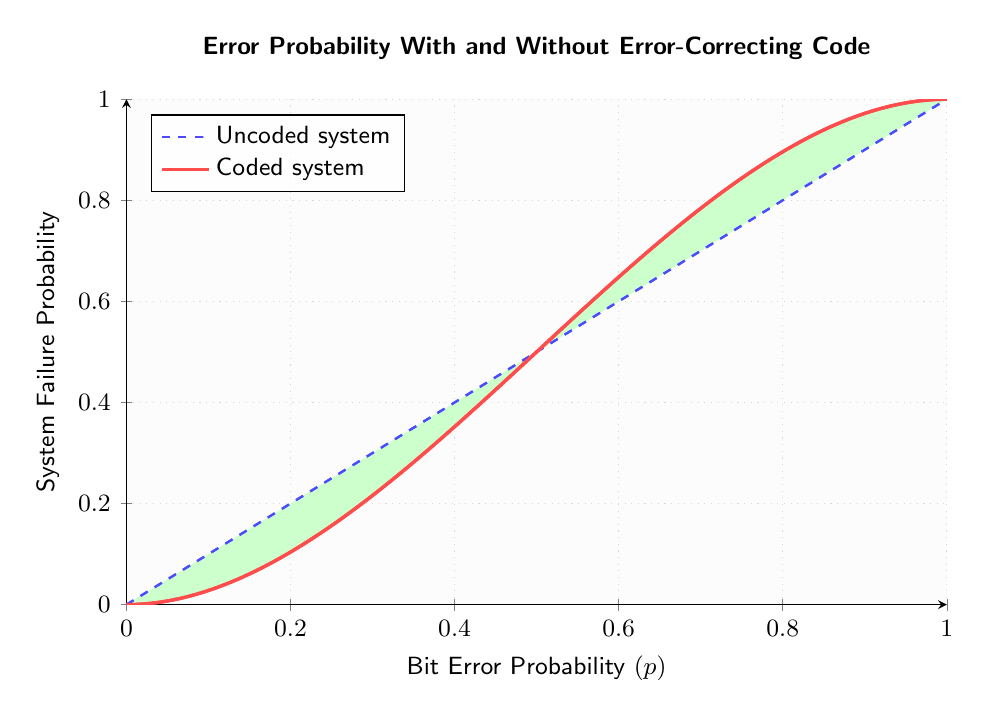
\begin{tikzpicture}[
    declare function={
        f(\x) = \x;
        g(\x) = 3*\x^2 - 2*\x^3;
    }
]
\begin{axis}[
    width=12cm,
    height=8cm,
    xlabel = {Bit Error Probability $(p)$},
    ylabel = {System Failure Probability},
    xlabel style={font=\small\sffamily},
    ylabel style={font=\small\sffamily},
    axis lines = left,
    xmin=0, xmax=1,
    ymin=0, ymax=1,
    xtick={0,0.2,0.4,0.6,0.8,1},
    ytick={0,0.2,0.4,0.6,0.8,1},
    tick label style={font=\small\sffamily},
    grid=major,
    grid style={dotted, gray!30},
    legend pos=north west,
    legend style={
        cells={anchor=west},
        font=\small\sffamily,
        fill=white,
        fill opacity=0.7,
        draw opacity=1,
        text opacity=1
    },
    samples=200,
    domain=0:1,
    smooth,
    title={\small\sffamily\bfseries Error Probability With and Without Error-Correcting Code},
    title style={yshift=5pt},
    axis background/.style={fill=gray!2}
]

\addplot[name path=f, dashed, blue!70, thick, forget plot] {f(x)};
\addplot[name path=g, solid, red!70, very thick, forget plot] {g(x)};

\addplot[green!20, forget plot] fill between[of=f and g];

\addplot[dashed, blue!70, thick] {f(x)};
\addplot[solid, red!70, very thick] {g(x)};

\legend{Uncoded system, Coded system}

\end{axis}
\end{tikzpicture}
\end{document}
